\documentclass[12pt]{amsart}
\usepackage{amsmath,amsthm,amssymb,amsfonts,enumerate,mymath,tikz-cd,fancyhdr}
\openup 5pt
\author{Blake Farman\\University of South Carolina}
\title{Math 116\\Exam 02}
\date{November 16, 2016}
\pdfpagewidth 8.5in
\pdfpageheight 11in
\usepackage[margin=1in]{geometry}

\renewcommand{\qedsymbol}{}
\graphicspath{ {../imgs/} }
\begin{document}
\maketitle

\begin{center}
  \fbox{\fbox{\parbox{5.5in}{\centering
        Answer the questions in the spaces provided on the
        question sheets and turn them in at the end of the class period.
        If you require extra space, use the back of the page and indicate that you have done so.
        
        Unless otherwise stated, all supporting work is required.
        Unsupported or otherwise mysterious answers will {\bf not receive credit.}
        You may {\it not} use any calculators.}}}
\end{center}

\vspace{0.2in}
\makebox[\textwidth]{Name:\enspace\hrulefill}
\vspace{0.2in}

$$
\begin{array}{|c|c|c|}
  \hline
  \text{Problem} & \text{Points Earned} & \text{Points Possible}\\
  \hline
  1 & & 20\\
  \hline
  2 & & 20\\
  \hline
  3 & & 20\\
  \hline
  4 & & 20\\
  \hline
  5 & & 20 \\
  \hline
  \text{Total} & & 100\\
  \hline
\end{array}
$$
\newpage

\theoremstyle{definition}
\newtheorem{thm}{}
\newtheorem{lem}{Lemma}
\theoremstyle{definition}
\newtheorem{defn}{Definition}

\begin{thm}[20 Points]\label{ex1}
  Find the period, frequency, and amplitude of $y = -2\sin\left(\frac{1}{2}x\right) + 2$, then graph one period.
  \begin{proof}[Solution]
    The amplitude is 2, the period is 
    $$\frac{2\pi}{\frac{1}{2}} = 2\pi \cdot \frac{2}{1} = 4\pi,$$
    and the frequency is 
    $$\frac{1}{4\pi}.$$
    \begin{enumerate}
    \item
      Plot $\sin(x)$:
      \begin{center}
        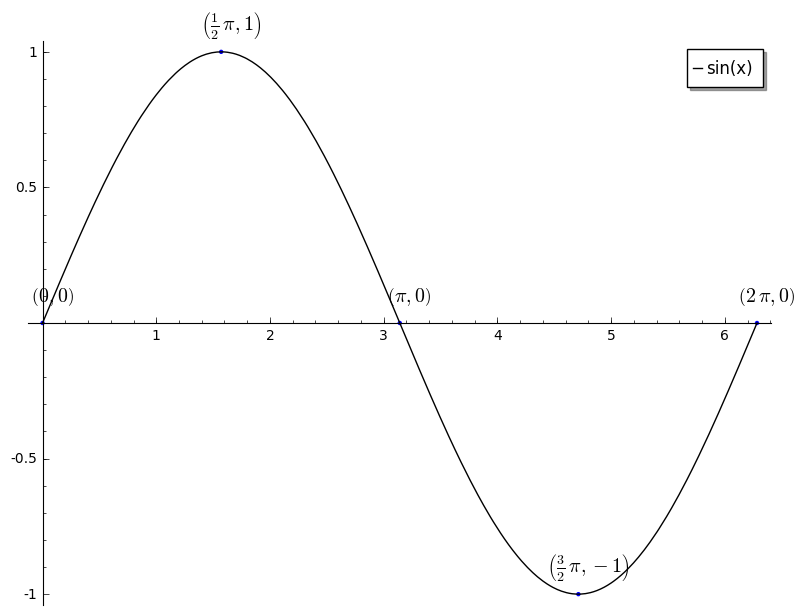
\includegraphics[scale=0.5]{sin/sine}
      \end{center}
    \item
      Stretch the graph of $\sin(x)$ horizontally by a factor of $2$ to obtain the graph of $\sin\left(\frac{1}{2}x\right)$:
      \begin{center}
        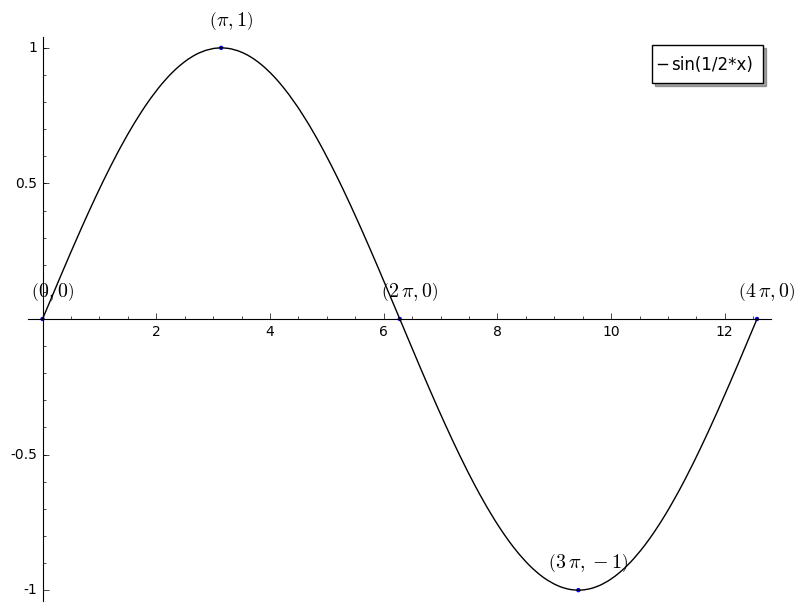
\includegraphics[scale=0.5]{sin/p_1}
      \end{center}
    \item
      Reflect the graph of $\sin\left(\frac{1}{2}x\right)$ across the $x$-axis to obtain the graph of $-\sin\left(\frac{1}{2}x\right)$:
      \begin{center}
        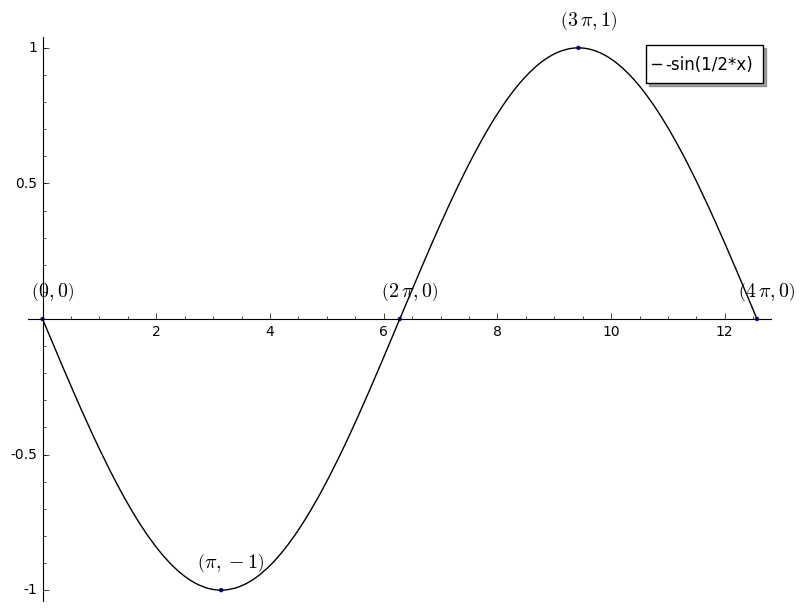
\includegraphics[scale=0.5]{sin/p_2}
      \end{center}
    \item
      Stretch the graph of $-\sin\left(\frac{1}{2}x\right)$ vertically by a factor of $2$ to obtain the graph of $-2\sin\left(\frac{1}{2}x\right)$:
      \begin{center}
        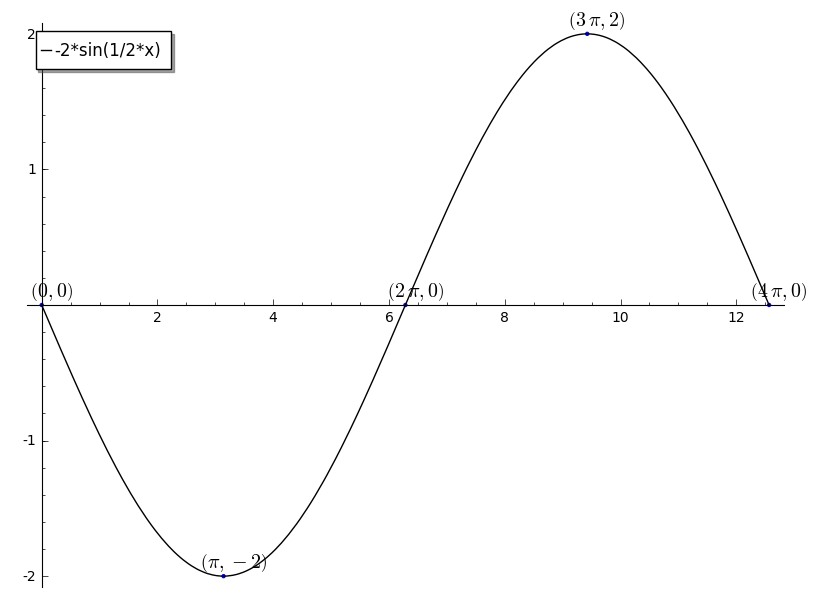
\includegraphics[scale=0.5]{sin/p_3}
      \end{center}
    \item
      Finally translate the graph of $-2\sin\left(\frac{1}{2}x\right)$ up by 2 to obtain the graph of $-2\sin\left(\frac{1}{2}x\right) + 2$:
      \begin{center}
        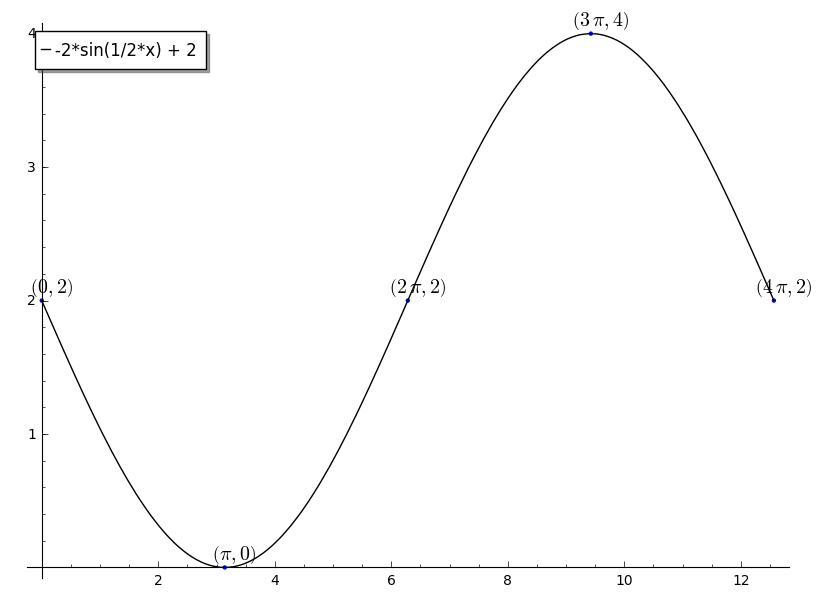
\includegraphics[scale=0.5]{sin/p_4}
      \end{center}
    \end{enumerate}
  \end{proof}
\end{thm}

\begin{thm}[20 Points]\label{ex2}
  Find the period, frequency, and amplitude of $y = 3\cos(4x) + 1$, then graph one period.
  
  \begin{proof}[Solution]
    The amplitude is 3, the period is
    $$\frac{2\pi}{4} = \frac{\pi/2},$$
    and the frequency is
    $$\frac{2}{\pi}.$$
    \begin{enumerate}
    \item
      Plot $\cos(x)$:
      \begin{center}
        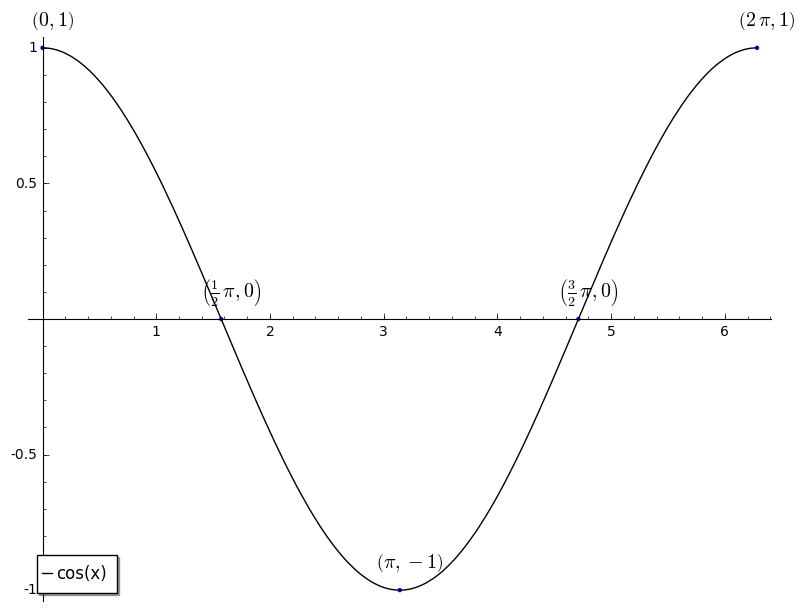
\includegraphics[scale=0.5]{cos/cos}
      \end{center}
    \item
      Compress the graph of $\cos(x)$ horizontally by a factor of 4 to obtain the graph of $\cos(4x)$:
      \begin{center}
        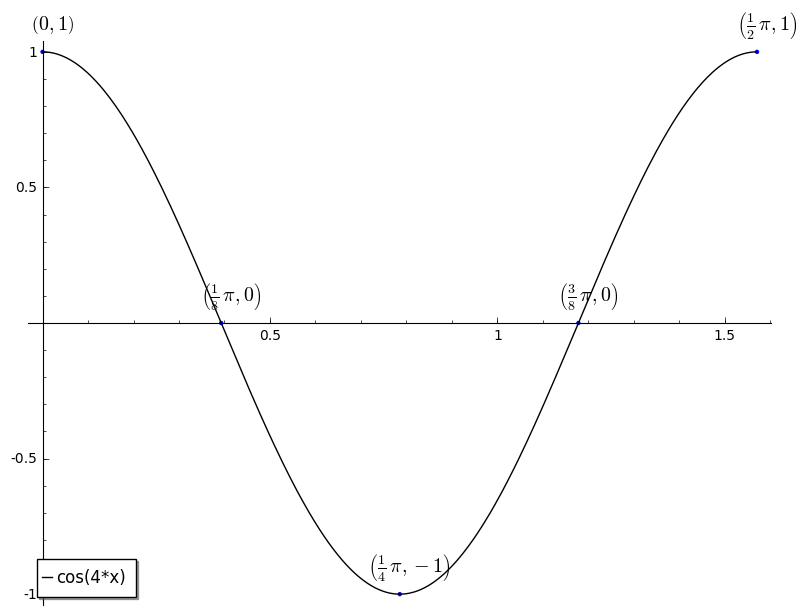
\includegraphics[scale=0.5]{cos/p_1}
      \end{center}
    \item
      Stretch the graph of $\cos(4x)$ vertically by a factor of 3 to obtain the graph of $3\cos(4x)$:
      \begin{center}
        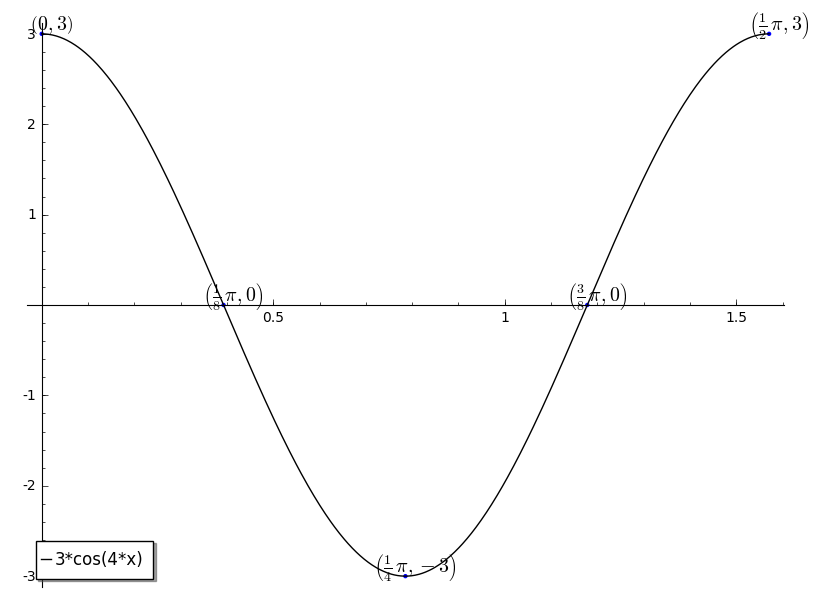
\includegraphics[scale=0.5]{cos/p_2}
      \end{center}
    \item
      Finally, translate the graph of $3\cos(4x)$ up by 1 to obtain the graph of $3\cos(4x) + 1$:
      \begin{center}
        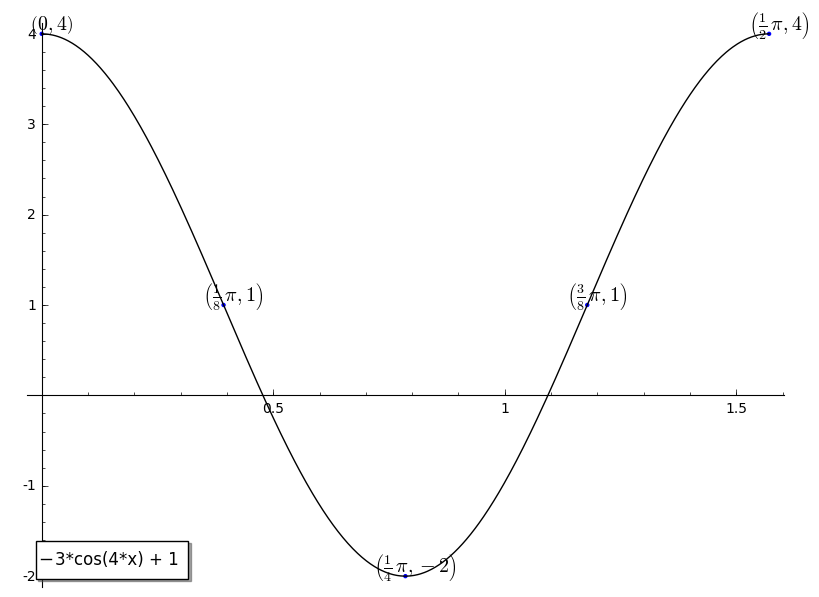
\includegraphics[scale=0.5]{cos/p_3}
      \end{center}
    \end{enumerate}
  \end{proof}
\end{thm}

\begin{thm}[20 Points]\label{ex3}
  Let $f(x) = x^2 - 1$ and $g(x) = x + 1$.
  \begin{enumerate}[(a)]
  \item
    Compute $(f \circ g)(x)$.
    \begin{proof}[Solution]
      \begin{eqnarray*}
        (f \circ g)(x) &=& f\left(g(x)\right)\\
        &=& f\left(x + 1\right)\\
        &=& (x + 1)^2 - 1\\
        &=& x^2 + 2x + 1 - 1\\
        &=& x^2 + 2x.
      \end{eqnarray*}
    \end{proof}
  \item
    Compute $(g \circ f)(x)$.
    \begin{proof}[Solution]
      \begin{eqnarray*}
        (g \circ f)(x) &=& g\left(f(x)\right)\\
        &=& g\left(x^2 - 1\right)\\
        &=& \left(x^2 - 1\right) + 1\\
        &=& x^2.
      \end{eqnarray*}
    \end{proof}
  \end{enumerate}
\end{thm}

\begin{thm}[20 Points]\label{ex4}
  Let $f(x) = x^3 - 1$ and $g(x) = x + 1$.
  \begin{enumerate}[(a)]
  \item
    Compute $f^{-1}(x)$.
    \begin{proof}[Solution]
      We solve $y = x^3 - 1$ for $x$. Adding one to both sides gives
      $$y + 1 = x^3$$
      and then taking the cube root of both sides gives
      $$x = \sqrt[3]{y + 1}.$$
      Therefore $f^{-1}(x) = \sqrt[3]{y + 1}$.
    \end{proof}
  \item
    Compute $g^{-1}(x)$.
    \begin{proof}[Solution]
      We solve $y = x + 1$ for $x$ to get $x = y - 1$.
      Therefore $g^{-1}(x) = x - 1$.
    \end{proof}
  \item
    Compute $(f \circ g)^{-1}(x)$.\\
    {\bf Hint}: You can compute this {\it without} computing $(f \circ g)(x)$.
    \begin{proof}[Solution]
      We note that by definition, we need only find a function that satisfies
      $$(f \circ g)^{-1} \circ (f \circ g)(x) = x$$
      and
      $$(f \circ g) \circ (f \circ g)^{-1}(x) = x.$$
      Since we have seen that $f$ and $g$ both have inverses, the composition $\left(g^{-1} \circ f^{-1}\right)(x)$ makes sense.
      Moreover,
      \begin{eqnarray*}
        \left(g^{-1} \circ f^{-1}\right) \circ (f \circ g)(x) &=&
        g^{-1}\left( f^{-1} \left(f\left( g(x)\right)\right)\right)\\
        &=& g^{-1}\left(g(x)\right)\\
        &=& x
      \end{eqnarray*}
      and
      \begin{eqnarray*}
        (f \circ g) \circ \left(g^{-1} \circ f^{-1}\right)(x) &=&
        f \left( g\left( g^{-1}\left( f^{-1}(x)\right)\right)\right)\\
        &=& f\left(f^{-1}(x)\right)\\
        &=& x.
      \end{eqnarray*}
      Therefore the inverse of $(f \circ g)(x)$ is
      \begin{eqnarray*}
        \left(g^{-1} \circ f^{-1}\right)(x) &=& g^{-1}\left(f^{-1}(x)\right)\\
        &=& g^{-1}\left(\sqrt[3]{x + 1}\right)\\
        &=& \left(\sqrt[3]{x + 1}\right) - 1.\\
      \end{eqnarray*}
    \end{proof}
  \end{enumerate}
\end{thm}

\begin{thm}[20 Points]\label{ex5}
  Solve the following equations for $x$.
  \begin{enumerate}[(a)]
  \item
    $$ \log_6(x-2) + \log_6(x - 3) = 1$$
    \begin{proof}[Solution]
      First combine the logarithms on the left-hand side to get the equation
      $$\log_6\left((x - 2)(x - 3)\right) = 1$$
      and then apply the exponential function $6^x$ to both sides to obtain
      $$6^{\log_6\left((x - 2)(x - 3)\right)} = 6^1 = 6.$$
      Since $6^x$ and $\log_6(x)$ are inverse functions we get the equation
      $$(x - 2)(x - 3) = 6.$$
      Subtracting 6 from both sides then expanding gives
      $$0 = (x^2 - 5x + 6) - 6 = x^2 - 5x = x(x - 5)$$
      and hence the possible solutions are $x = 5$ and $x = 0$.
      The solution $x = 0$ is extraneous because $\log_6(0 - 2) = \log_6(-2)$ and $\log_6(0 - 3) = \log_6(-3)$ are both undefined.
      Therefore the only solution is $x = 5$.
    \end{proof}
  \item
    $$e^{2x} - 1 = 0$$
    \begin{proof}[Solution 1]
      Rewrite $e^{2x}$ as $\left(e^x\right)^2$ and then factor the left-hand side to get
      $$\left(e^x + 1)\right(e^x - 1) = 0$$
      which implies either $e^x = 1$ or $e^x = -1$.
      The former implies that $x = 0$ and the latter has no solution because $e^x$ is {\it always} positive.
      Therefore $x = 0$.
    \end{proof}
    \begin{proof}[Solution 2]
      Add 1 to both sides to obtain
      $$e^{2x} = 1$$
      and the apply $\ln(x)$ to both sides to get
      $$2x = \ln(e^{2x}) = \ln(1) = 0$$
      and hence $x = 0$.
    \end{proof}
  \end{enumerate}
\end{thm}
\end{document}
